% !TeX root = main.tex
\documentclass[12pt,a4paper,openany,twoside,below,section]{book}

% ======= 页面和版面设置 =======
\usepackage{geometry}   % 设置页边距
\geometry{paperwidth=210mm,paperheight=297mm,%
  left=2.5cm,right=2.5cm,top=2.54cm,bottom=2.54cm}
\topmargin=-10.4mm
\headheight=17pt
\footskip=8mm
\headsep=5mm

\usepackage[below]{placeins}  % 防止浮动体跨越章节
\usepackage{float}  % 图片浮动位置控制

% ======= 图形和表格 =======
\usepackage{graphicx}  % 插图
\graphicspath{{figures/}}  % 预定义图片路径
\usepackage{subfigure}  % 多子图支持
\usepackage{rotating}  % 旋转图形
\usepackage{tabularx}  % 表格扩展
\usepackage{multirow}  % 表格多行合并
\usepackage{setspace}  % 行距设置
\usepackage[ruled,linesnumbered]{algorithm2e}
\usepackage{booktabs}  % 绘制三线表
\setlength\heavyrulewidth{0.35ex}

% ======= 文字编码和字体 =======
\usepackage{fontspec,xltxtra,xunicode}
\defaultfontfeatures{Mapping=tex-text} % 支持连字符等特殊符号
\usepackage{xeCJK}  % 中文支持
\usepackage{ctex}

% 中文字体配置
\setmainfont{Times New Roman}
\setsansfont{Times New Roman}
\setmonofont{Courier New}
\setCJKmainfont[AutoFakeBold=true]{SimSun}  % 宋体
\setCJKsansfont{SimHei}
\setCJKmonofont{FangSong}

\setCJKfamilyfont{hei}{SimHei}               % 黑体
\setCJKfamilyfont{kai}{KaiTi}                % 楷体
\setCJKfamilyfont{song}[AutoFakeBold]{SimSun}  % 宋体
\setCJKfamilyfont{fang}{FangSong}            % 仿宋体
\setCJKfamilyfont{enroman}{Times New Roman}

\newcommand{\hei}{\CJKfamily{hei}}
\newcommand{\kai}{\CJKfamily{kai}}
\newcommand{\song}{\CJKfamily{song}}
\newcommand{\fang}{\CJKfamily{fang}}
\newcommand*{\mytimes}{\CJKfamily{enroman}}

\newfontfamily\codefont{Courier New}
\newfontfamily\pagella{Times New Roman}

% ======= 字号、行距定义 =======
\newcommand{\yihao}{\fontsize{28pt}{36pt}\selectfont}     % 一号
\newcommand{\erhao}{\fontsize{21pt}{28pt}\selectfont}     % 二号
\newcommand{\sanhao}{\fontsize{16pt}{20pt}\selectfont}    % 三号
\newcommand{\xiaosan}{\fontsize{15pt}{22pt}\selectfont}   % 小三
\newcommand{\sihao}{\fontsize{14pt}{20pt}\selectfont}     % 四号
\newcommand{\xiaosi}{\fontsize{12pt}{20pt}\selectfont}    % 小四
\newcommand{\wuhao}{\fontsize{10.5pt}{10.5pt}\selectfont} % 五号
\newcommand{\xiaowu}{\fontsize{9pt}{9pt}\selectfont}      % 小五

\renewcommand{\baselinestretch}{1.0}  % 将行距缩放系数设为1,避免中文默认1.3导致的行距放大,使设定的20pt行距实际生效(否则为26pt),需配合 \selectfont 使用

% ======= 颜色和超链接 =======
\usepackage{xcolor}
\usepackage{color}  % 也可删除,xcolor已包含
\usepackage[unicode]{hyperref}
\hypersetup{
  hidelinks,
  CJKbookmarks=true,
  bookmarksnumbered=true,
  bookmarksopen=true,
  colorlinks=true,
  pdfborder=001,
  citecolor=blue,
  linkcolor=blue,
  anchorcolor=green,
  urlcolor=blue,
  pdfcreator={XeTeX,XeCJK}
}

\usepackage{caption}
%按NWPU标准, 图表标题字号为五号
\DeclareCaptionFont{tiZhuZiTi}{\fontsize{10.5}{10.5}\mdseries}
% 按NWPU标准, 设置题注分隔符
\DeclareCaptionLabelSeparator{tiZhuFenGe}{\hspace{0.5em}}
%重新定义caption的属性
\captionsetup{font=tiZhuZiTi, labelsep=tiZhuFenGe, skip=10pt}

% ======= 参考文献 =======
\usepackage[numbers,super,square,comma,sort&compress]{natbib}

% ======= 代码、下划线等特殊格式 =======
\usepackage{listings}  % 代码插入
\usepackage{ulem}      % 下划线、波浪线等

% ======= 画图 =======
\usepackage{tikz}

% ======= 其他 =======
\usepackage{wallpaper}  % 背景图片
\addtolength{\wpYoffset}{8.0cm}
\usepackage{url}
\usepackage{epsfig}     % eps图像支持
\usepackage{flafter}    % 浮动体显示顺序
\usepackage{calc}       % 计算
\usepackage{units}      % 单位宏包

% ======= 数学符号 =======
\usepackage{amsmath,amssymb}
\usepackage{mathtools}
\usepackage{bm}  % 粗斜体

% ======= 行距与段落设置 =======
% \linespread{1.4}
% \setlength{\parskip}{0.5\baselineskip}
\sloppy

% 段落首行缩进2个中文字符
\makeatletter
\let\@afterindentfalse\@afterindenttrue
\@afterindenttrue
\makeatother
\setlength{\parindent}{2em}

% ======= 页眉页脚 =======
\usepackage{fancyhdr}
\pagestyle{fancy}
\fancyhf{}  % 清空默认
\fancyfoot[C]{\thepage}  % 页脚居中显示页码
\renewcommand{\headrulewidth}{0pt}  % 去掉页眉线
\renewcommand{\footrulewidth}{0pt}  % 去掉页脚线

% ======= 图表编号按章节 =======
\usepackage{chngcntr}
\counterwithin{figure}{chapter}
\counterwithin{table}{chapter}
\counterwithin{equation}{chapter}
\renewcommand{\thefigure}{\thechapter-\arabic{figure}}
\renewcommand{\thetable}{\thechapter-\arabic{table}}
\renewcommand{\theequation}{\thechapter-\arabic{equation}}

% ======= 章节标题格式 =======
\setcounter{secnumdepth}{4}
\input{setup/gb_452.cpx}
\renewcommand\chaptername{\CJKprechaptername\CJKthechapter\CJKchaptername}



\usepackage{titlesec}

\titleformat{\chapter}[hang]
    {\filcenter \hei \fontsize{16pt}{20pt}\selectfont}
    {\hei \fontsize{16pt}{20pt}\selectfont{\chaptertitlename}}
    {16pt}{}
\titlespacing{\chapter}{0pt}{-2pt}{14pt}


\titleformat{\section}[hang]{\hei \sihao}
  {\sihao \thesection}{0.5em}{}
\titlespacing{\section}{0pt}{10pt}{0em}

\titleformat{\subsection}[hang]{\hei \xiaosi}
  {\xiaosi \thesubsection}{0.5em}{}
\titlespacing{\subsection}{0pt}{10pt}{0em}

% ======= 目录格式修改 =======
\usepackage{etoolbox}
\usepackage{titletoc}

\setcounter{tocdepth}{2}
\renewcommand{\contentsname}{目~~~~录}
\dottedcontents{chapter}[0.0em]{}{0.0em}{5pt}
\dottedcontents{section}[1.16cm]{}{1.8em}{5pt}
\dottedcontents{subsection}[2.00cm]{}{2.7em}{5pt}

\raggedbottom
% 调整列表环境的垂直间距和水平缩进
% labelindent=26pt, 两个小四字符是2*12pt=24pt,再修正2pt以求避免编号数字有突出感。下同。
\usepackage{enumitem}
\setlist[enumerate]{itemsep=0pt, topsep=0pt, partopsep=0pt, parsep=0pt,
                    labelindent=26pt, leftmargin=*, align=left}
\setlist[itemize]{itemsep=2pt, topsep=2pt, partopsep=2pt, parsep=2pt}
                %  labelindent=26pt, leftmargin=*, align=left}
\setlist[description]{itemsep=0pt, topsep=0pt, partopsep=0pt, parsep=0pt,
                      labelindent=26pt, leftmargin=*, align=left}

% 设置中文风格的章节引用
\newcommand{\chref}[1]{\CJKnumber{\ref{#1}}}
% 调整中文括号的间距
\newcommand{\KH}[1]{\!\!(#1)\!\!}
% 重设表格的纵向尺寸
\renewcommand\arraystretch{1.25}

% ======= 注释掉的示例标题格式 =======
% \title{\yihao{这里是大标题啊}}
% \author{\xiaoerhao{作者姓名}\footnote{电子邮件: ***@***.com,学号: ***}\\[2ex]
% \sanhao 东南大学网络空间安全学院\\[2ex]
% }
% \date{\sanhao\today}


\let\cleardoublepage\clearpage


% ==== 标题、作者、日期信息 ====
\title{\yihao{标题}\\[20ex]}
\author{
    \erhao{作者}
    \thanks{电子邮件: XXXX@mail.nwpu.edu.cn}\\[2ex]
    \sanhao XX大学XX学院\\[2ex]
}
% \date{\sanhao\today}
\date{\sanhao XXXX年X月X日}


\begin{document}
\renewcommand{\thefootnote}{}  % 禁用脚注序号
\xiaosi\song  % 定义默认字体
\renewcommand{\d}{\mathrm{d}}  % 微分正体
\frontmatter % 前置部分页码采用罗马数字

% 封面页(不分页,不显示页码)
\begingroup
\let\newpage\relax  % 防止 \maketitle 后自动换页
\thispagestyle{empty}  % 不显示页码
\maketitle
\endgroup

\newpage
\setcounter{page}{1}  % 第二页从页码1开始


% {{{ ==== 摘要 ====
\phantomsection  % 生成锚点,供目录和超链接引用
\chapter*{摘~~~~要}
\markboth{摘~~~~要}{摘~~~~要}
\addcontentsline{toc}{chapter}{摘~~~~要}  % 添加到目录
摘要内容……

\vspace{1em}
\noindent {\hei 关键词:} \quad 词1,词2,词3,词4,词5

\newpage
% }}}


% ==== 目录 ====
\phantomsection
\addcontentsline{toc}{chapter}{目~~~~录}
\tableofcontents

\mainmatter  % 主体部分页码采用阿拉伯数字


% ==== 正文章节 ====
% {{{ chapter1
\chapter{我是第1章}
第一章内容。

\begin{equation}
\left( \frac{\delta_n}{\delta_{no}} \right)^2 + \left( \frac{\delta_t}{\delta_{so}} \right)^2 = 1
\label{eq:damage_initiation}
\end{equation}
其中,$\delta_n$ 与 $\delta_t$ 分别为法向和切向开裂位移,$\delta_{no}$ 与 $\delta_{so}$ 为对应的初始损伤位移阈值。

假设切向位移可表示为 $\delta_t = \beta \delta_n$,其中
\begin{equation}
\beta = \frac{\sqrt{\delta_{t1}^2 + \delta_{t2}^2}}{\delta_n}
\label{eq:beta_def}
\end{equation}
代入式 \eqref{eq:damage_initiation} 可得:
\begin{equation}
\left( \frac{\delta_n}{\delta_{no}} \right)^2 + \left( \frac{\beta \delta_n}{\delta_{so}} \right)^2 = 1
\end{equation}
整理得到:
\begin{equation}
\delta_n^2 \left( \frac{1}{\delta_{no}^2} + \frac{\beta^2}{\delta_{so}^2} \right) = 1
\quad \Rightarrow \quad
\delta_n^2 = \frac{1}{\frac{1}{\delta_{no}^2} + \frac{\beta^2}{\delta_{so}^2}} = \frac{\delta_{no}^2 \delta_{so}^2}{\delta_{so}^2 + \delta_{no}^2 \beta^2}
\end{equation}

此时的等效初始位移 $\delta_{mo}$ 可表示为:
\begin{equation}
\delta_{mo}^2 = \delta_n^2 + \delta_t^2 = \delta_n^2(1 + \beta^2)
\end{equation}
最终得到混合模式下的等效初始位移为:
\begin{equation}
\delta_{mo} = \delta_{no} \delta_{so} \sqrt{ \frac{1 + \beta^2}{\delta_{so}^2 + \delta_{no}^2 \beta^2} }
\label{eq:delta_mo}
\end{equation}

\section{一章一节}
内容……

\begin{figure}[H] %H为当前位置,!htb为忽略美学标准,htbp为浮动图形
    \centering %图片居中
    
\includegraphics[width=0.5\textwidth]{example1.jpeg} %插入图片,[]中设置图片大小,{}中是图片文件名
    \caption{Main name} %最终文档中希望显示的图片标题
    \label{Fig.main1} %用于文内引用的标签
    \end{figure}
% }}}

% {{{ chapter2
\chapter{我是第2章}
\section{二章一节}
文献\cite{li2023deep1,li2023deep2,li2023deep3},真的\cite{li2023deep1}叙述了……

图\ref{Fig.sub.1},图\ref{Fig.sub.2},图\ref{Fig.sub.3}如下所示:
\begin{figure}[H]
\centering  %图片全局居中
\subfigure[name1]{
\label{Fig.sub.1}

\includegraphics[width=0.3\textwidth]{example1.jpeg}}
\subfigure[name2]{
\label{Fig.sub.2}

\includegraphics[width=0.3\textwidth]{example2.jpeg}}
\subfigure[name3]{
\label{Fig.sub.3}
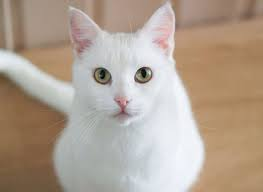
\includegraphics[width=0.3\textwidth]{example3.jpeg}}
\caption{Main name}
\label{Fig.main2}
\end{figure}

这是一个三线表。
\begin{table}[hbt!]
    \small
    \caption{\label{Tab5:table_aging_ASTM} 力学试验标准及试件尺寸}
    \centering
    \begin{tabularx}{\textwidth}{XXX c}
    \toprule
    试验 & 参考标准 & 试件尺寸(mm) & 加载速率(mm/min) \\
    \midrule
    弯曲试验     & ASTM-D7264 & $\text{95.0}\times \text{10.0}\times \text{2.0}$ & 1.0\\
    短梁剪切试验  & ASTM-D2344 & $\text{6.0}\times \text{4.0}\times \text{2.0}$ & 1.0\\
    双悬臂梁试验  & ASTM-D5528 & $\text{150.0}\times \text{25.0}\times \text{2.0}$ & 2.0\\
    \bottomrule
    \end{tabularx}
\end{table}
% }}}

% ==== 参考文献 ====
\begingroup
  % \cleardoublepage
  \phantomsection
  \addcontentsline{toc}{chapter}{参考文献}
  \bibliographystyle{references/gbt7714-2005}
  \xiaosi\song
  \setlength{\bibsep}{5pt}
  \setstretch{1.15}
  \bibliography{references/Library}
\endgroup

\end{document}
